\subsection{Architecture}
The Robotutors presentations are based on scripts. These are human made files containting the text of the presentation. This text is synthesised to to speech by the NAO's engine during the presenation. Additonally the text also contains a number of commands. These are actions the robot will perform during the lecture, such as its movements. The pacing of the slideshow is also controlled using these commands.\\
During the presentation, two pieces of software ensure the execution of the script. One part runs on the NAO itself, another on the computer that is used for the presentation. The computer is connected to the beamer or screen and runs the slideshow. This computer is also used to load, start and pause the script. The script is interpreted on the NAO. Here the text is being synthesized and the commands executed.

\begin{figure}
	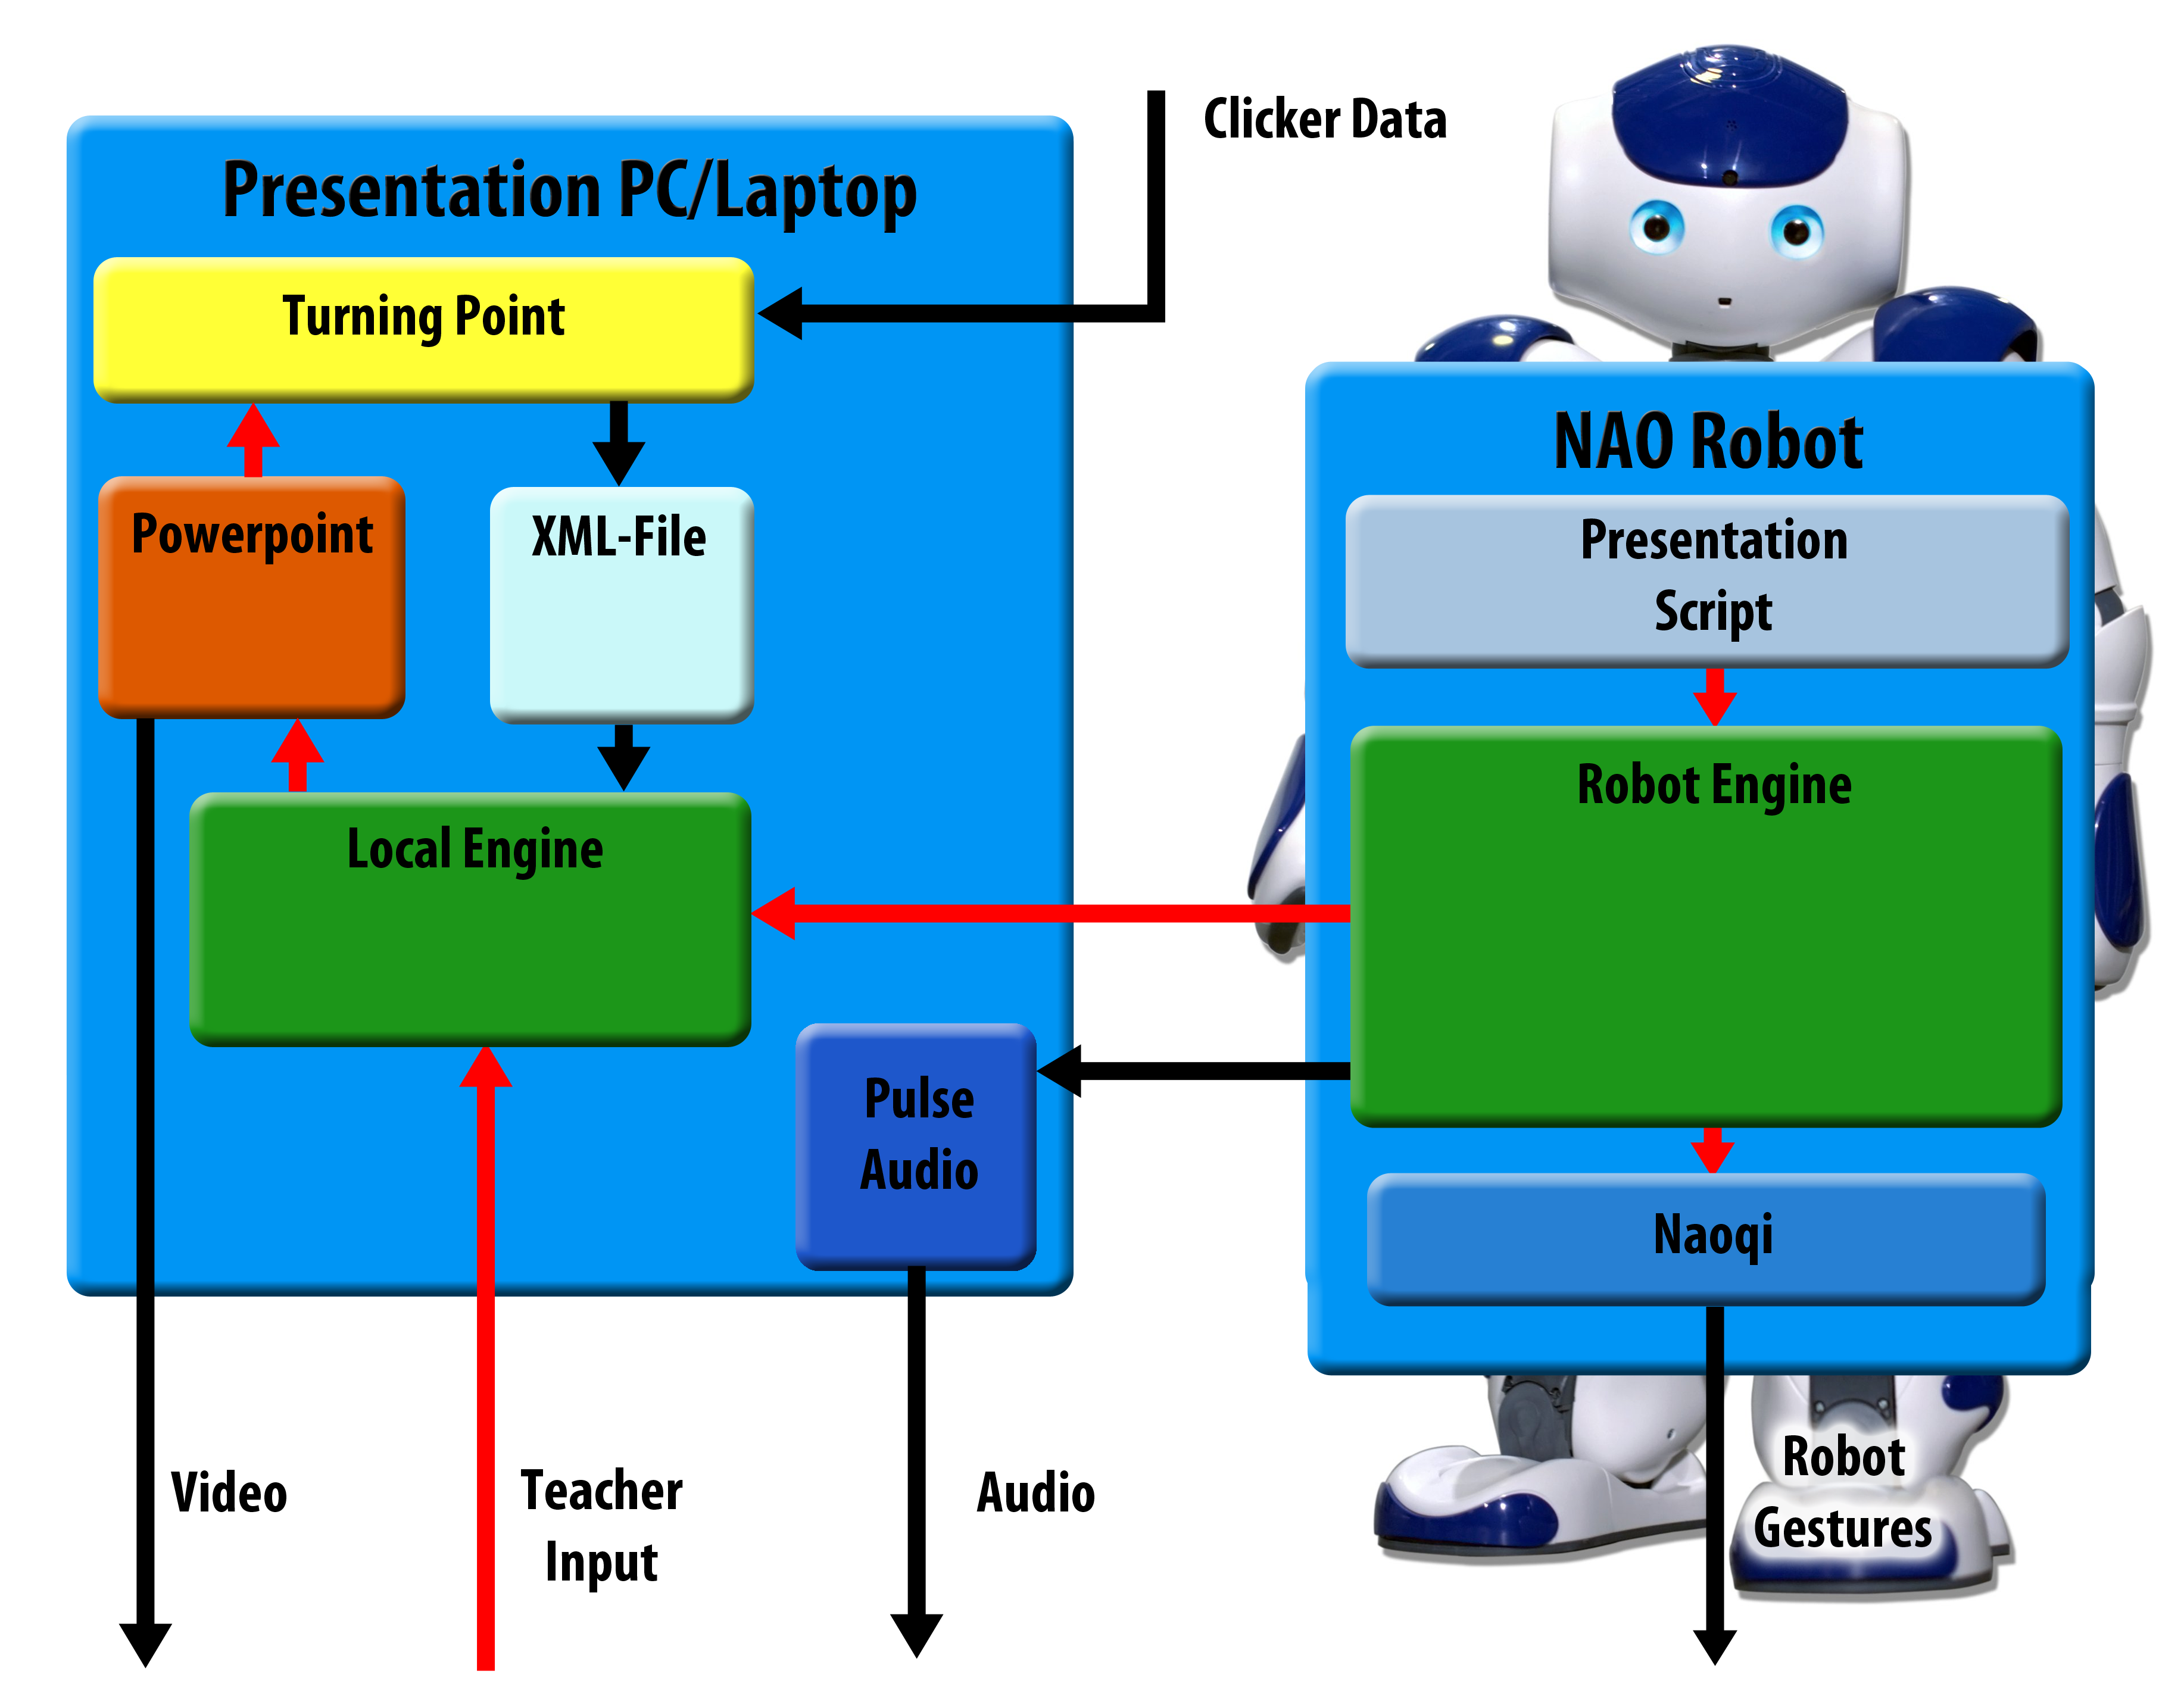
\includegraphics[scale=0.1]{images/system_overview.png}
	\caption{System overview}
\end{figure}

%C++, Script Engine

\subsection{Features}
\subsubsection{Powerpoint}
The robot can go to the next slide, step back or forward a specific number of slide, or go to a certain slide. Additonally, slide with new content can be dynamically created.

\subsubsection{Turningpoint}
The Turningpoint system consists of a number of response cards, small electronic devices, connected to a computer. The response card are handed out to people in the audience, who can use them to digitally respond to a question. Turningpoint then aggregates and presents the results. This can be used by a lecturer to check the audiences opinon or knowledge. The use of this technology is integrated into the Robotutor system. Using it, the NAO can ask questions and interpret the results. This provides a great method for interaction with the audience.

\subsubsection{Pulse Audio}
In large rooms or lecture halls, the NAO's internal speakers might not have enough volume to server the audience properly. For these kind of situations audio streaming has been implemented. Using pulse audio, the NAO's sound can be redirected to a different set of speakers.
